\documentclass[12pt, a4paper]{article}
\usepackage{array}
\usepackage{graphicx}
\usepackage{longtable}
\usepackage{etoolbox}

\setlength{\parindent}{0em}
\setlength{\parskip}{1em}

\newcounter{rowcntr}[table]
\renewcommand{\therowcntr}{\thetable.\arabic{rowcntr}}
% A new columntype to apply automatic stepping
\newcolumntype{N}{>{\refstepcounter{rowcntr}\therowcntr}c}
% Reset the rowcntr counter at each new tabular
\AtBeginEnvironment{tabular}{\setcounter{rowcntr}{0}}

\begin{document}

%\section{List of Tables}
\listoftables

\section{Background and Literature Review}
\subsection{Survey of online methods for changing and matching skin colour in Photoshop}
%TODO text

\section{Methods}
We tested progressive iterations of the algorithm on a set of hand images with varying skintones. The images are as follows:
%TODO The different hand images and their average skin colours. The masks used to obtain the area used to find the average skin colours of the hand can be found on the github repo for this project, under inputs/

We iterated from simple to more complex algorithms, at each step testing the algorithm on the hand images and evaluating the results. For each test, we call the recolor program to transform the image of one hand to have the skintone of the hand in another image. We perform the transformation, for each iteration of the algorithm, on all possible combinations of our test images, paying particular attention to the extreme cases as well as cases that start with a midtoned hand (as this is the most likely use case for applications that change a model's hand to match a range of skintones). We evaluate the resulting images subjectively, based on whether the processed hand looks believably like a hand naturally of that skintone, and note any flaws that we attempt to correct with the next iteration of the algorithm.

Below we summarize the results of each algorithm and our evaluation of the results.

\subsection{Simple brightness addition / subtraction}
%TODO text
See Appendix for full results.

\subsection{Proportional adjustment relative to average color}
%TODO text
See Appendix for full results.

\pagebreak

\section*{Appendix}
\begin{longtable}{|N||c|c|c|}
	\caption{Test results for xx.\label{tab:results_xx}}\\
	\hline
	\multicolumn{1}{|c||}{No.} & Original & Target & Results \\ 
	\hline
	  \label{row:results_xx_1} &
    \begin{minipage}{.29\textwidth}
      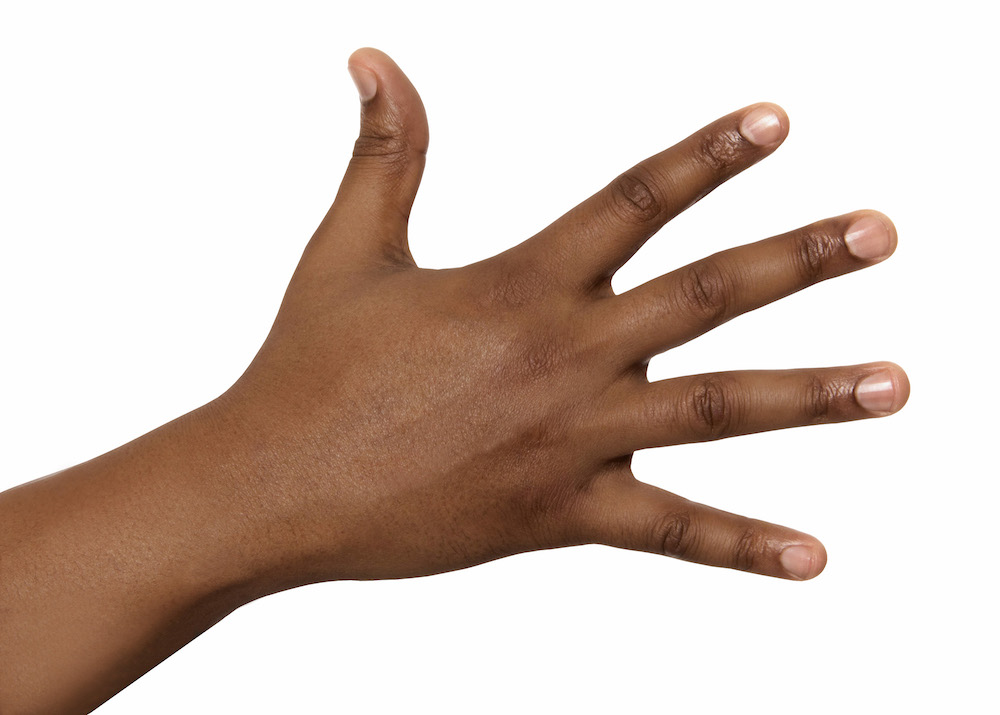
\includegraphics[width=\textwidth,height=\textheight,keepaspectratio]{images/test/hand_dark}
    \end{minipage} & 
    \begin{minipage}{.29\textwidth}
      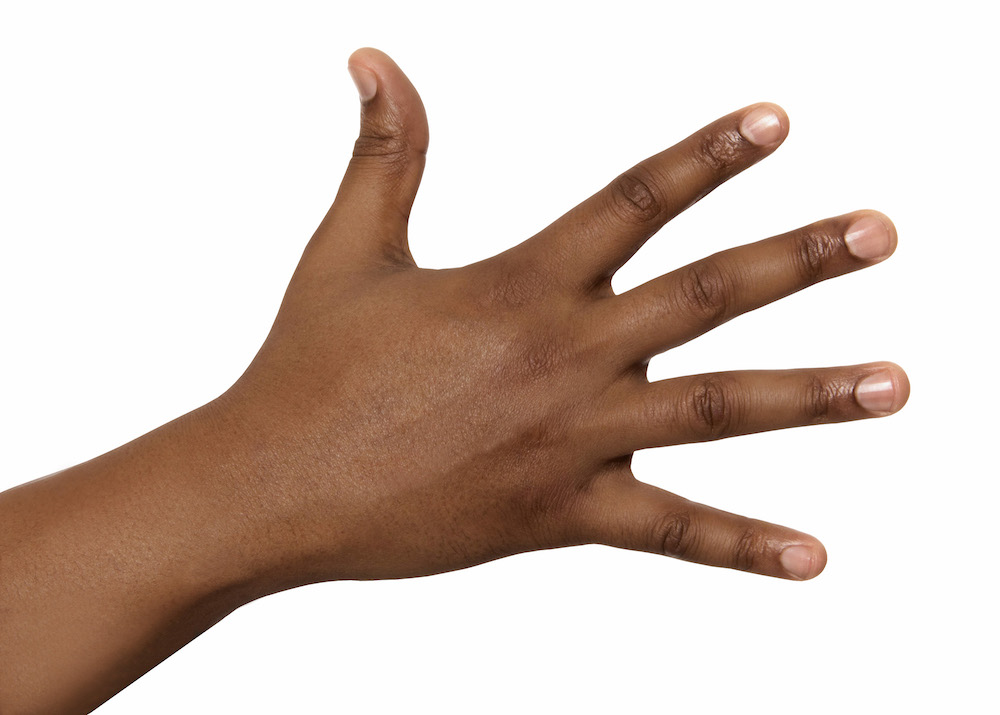
\includegraphics[width=\textwidth,height=\textheight,keepaspectratio]{images/test/hand_dark}
    \end{minipage} & 
    \begin{minipage}{.29\textwidth}
      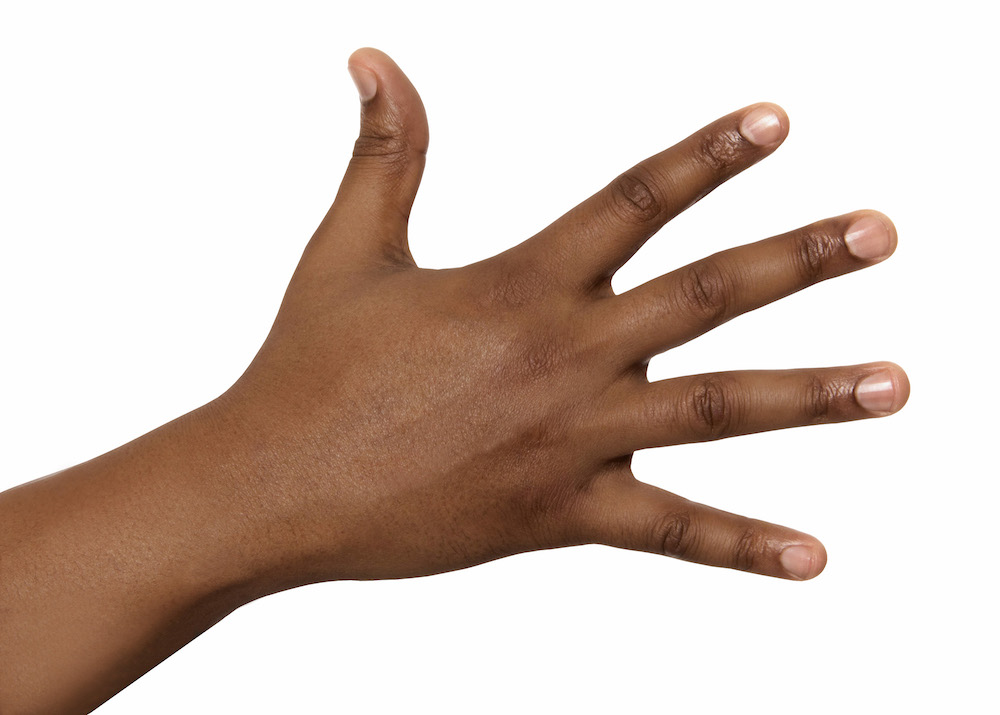
\includegraphics[width=\textwidth,height=\textheight,keepaspectratio]{images/test/hand_dark}
    \end{minipage} \\
  \hline
    \label{row:results_xx_2} &
    \begin{minipage}{.29\textwidth}
      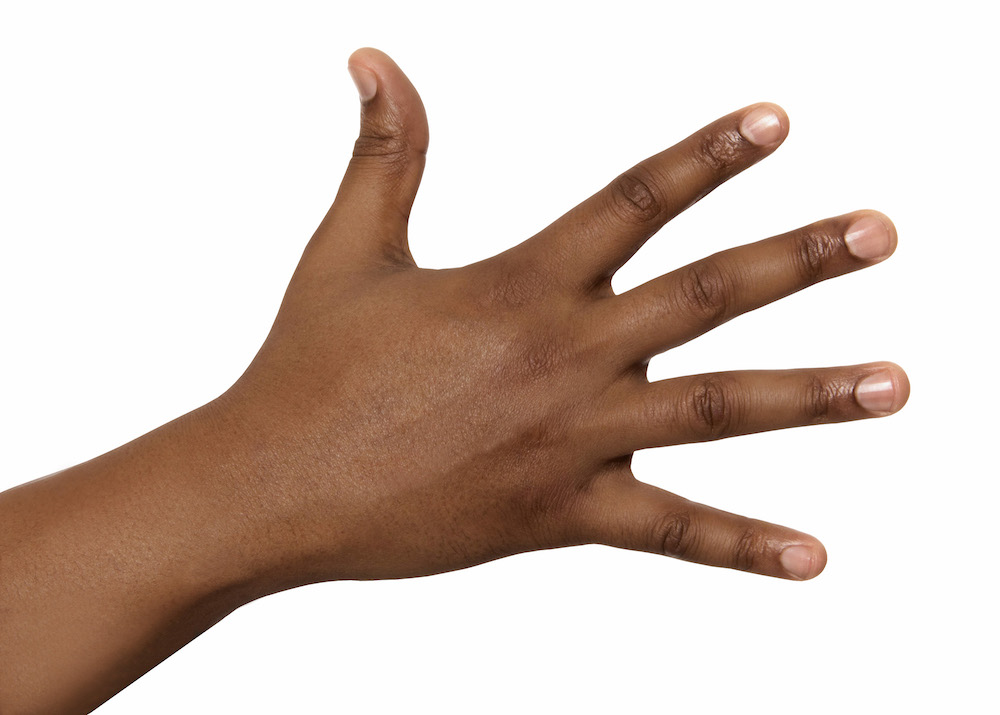
\includegraphics[width=\textwidth,height=\textheight,keepaspectratio]{images/test/hand_dark}
    \end{minipage} & 
    \begin{minipage}{.29\textwidth}
      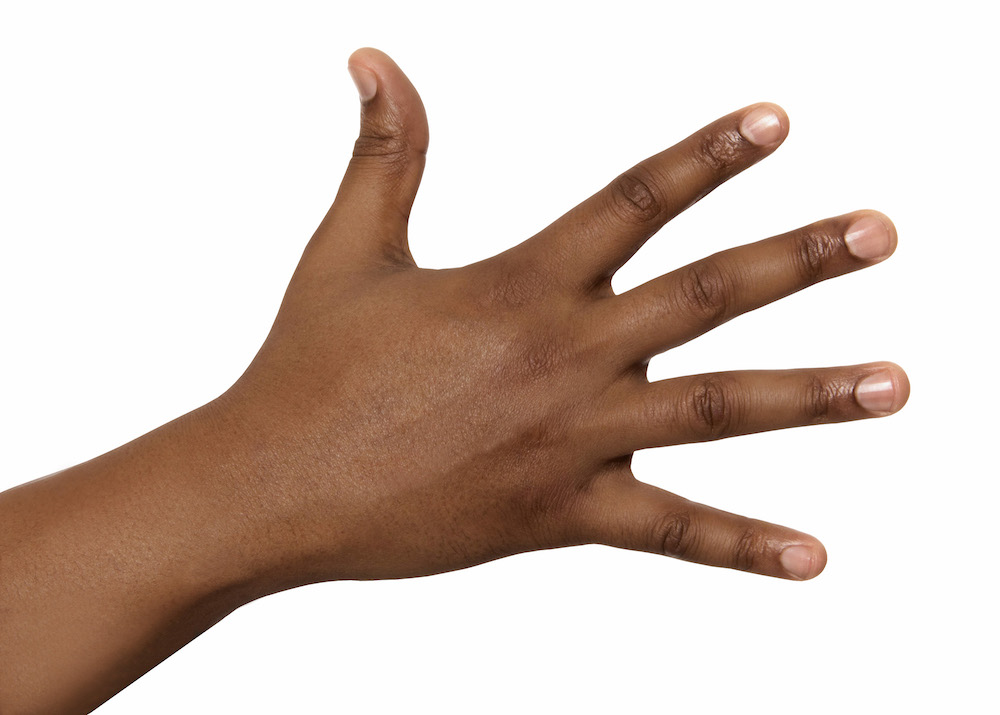
\includegraphics[width=\textwidth,height=\textheight,keepaspectratio]{images/test/hand_dark}
    \end{minipage} & 
    \begin{minipage}{.29\textwidth}
      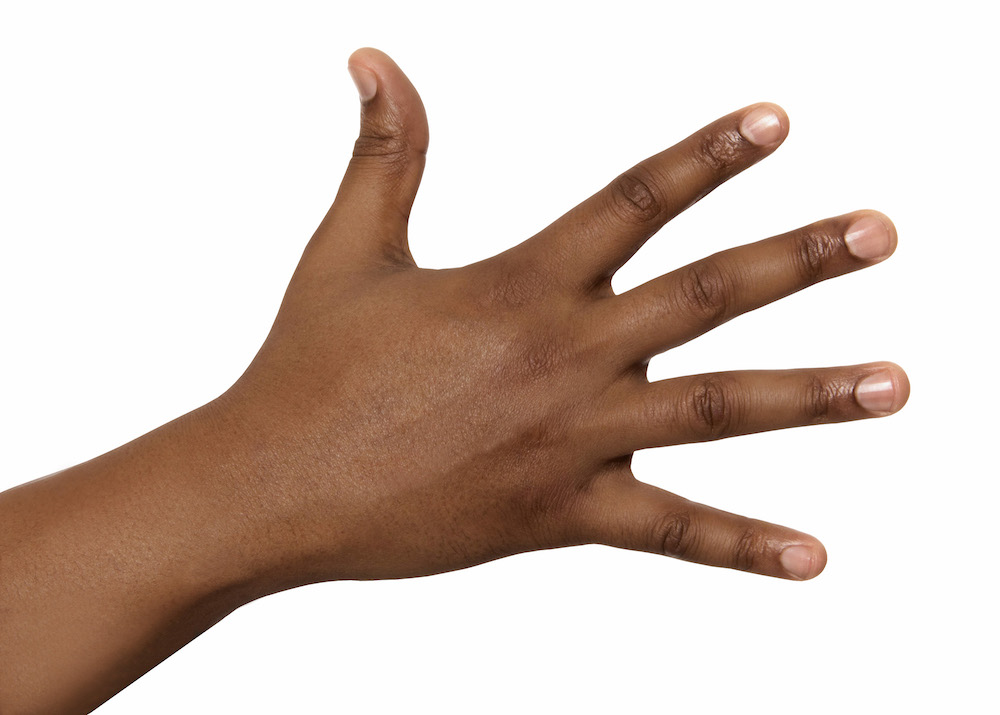
\includegraphics[width=\textwidth,height=\textheight,keepaspectratio]{images/test/hand_dark}
    \end{minipage} \\
  \hline
 \end{longtable}

\end{document}